\documentclass[10pt]{article}\usepackage[]{graphicx}\usepackage[]{xcolor}
% maxwidth is the original width if it is less than linewidth
% otherwise use linewidth (to make sure the graphics do not exceed the margin)
\makeatletter
\def\maxwidth{ %
  \ifdim\Gin@nat@width>\linewidth
    \linewidth
  \else
    \Gin@nat@width
  \fi
}
\makeatother

\definecolor{fgcolor}{rgb}{0.345, 0.345, 0.345}
\newcommand{\hlnum}[1]{\textcolor[rgb]{0.686,0.059,0.569}{#1}}%
\newcommand{\hlstr}[1]{\textcolor[rgb]{0.192,0.494,0.8}{#1}}%
\newcommand{\hlcom}[1]{\textcolor[rgb]{0.678,0.584,0.686}{\textit{#1}}}%
\newcommand{\hlopt}[1]{\textcolor[rgb]{0,0,0}{#1}}%
\newcommand{\hlstd}[1]{\textcolor[rgb]{0.345,0.345,0.345}{#1}}%
\newcommand{\hlkwa}[1]{\textcolor[rgb]{0.161,0.373,0.58}{\textbf{#1}}}%
\newcommand{\hlkwb}[1]{\textcolor[rgb]{0.69,0.353,0.396}{#1}}%
\newcommand{\hlkwc}[1]{\textcolor[rgb]{0.333,0.667,0.333}{#1}}%
\newcommand{\hlkwd}[1]{\textcolor[rgb]{0.737,0.353,0.396}{\textbf{#1}}}%
\let\hlipl\hlkwb

\usepackage{framed}
\makeatletter
\newenvironment{kframe}{%
 \def\at@end@of@kframe{}%
 \ifinner\ifhmode%
  \def\at@end@of@kframe{\end{minipage}}%
  \begin{minipage}{\columnwidth}%
 \fi\fi%
 \def\FrameCommand##1{\hskip\@totalleftmargin \hskip-\fboxsep
 \colorbox{shadecolor}{##1}\hskip-\fboxsep
     % There is no \\@totalrightmargin, so:
     \hskip-\linewidth \hskip-\@totalleftmargin \hskip\columnwidth}%
 \MakeFramed {\advance\hsize-\width
   \@totalleftmargin\z@ \linewidth\hsize
   \@setminipage}}%
 {\par\unskip\endMakeFramed%
 \at@end@of@kframe}
\makeatother

\definecolor{shadecolor}{rgb}{.97, .97, .97}
\definecolor{messagecolor}{rgb}{0, 0, 0}
\definecolor{warningcolor}{rgb}{1, 0, 1}
\definecolor{errorcolor}{rgb}{1, 0, 0}
\newenvironment{knitrout}{}{} % an empty environment to be redefined in TeX

\usepackage{alltt}
\usepackage[left=1in,right=1in,top=1in,bottom=1in]{geometry}
\usepackage{amsmath}
\usepackage{hyperref}
\usepackage{float}

\begin{knitrout}
\definecolor{shadecolor}{rgb}{0.969, 0.969, 0.969}\color{fgcolor}\begin{kframe}


{\ttfamily\noindent\bfseries\color{errorcolor}{\#\# Error in library(tidyverse): there is no package called 'tidyverse'}}\end{kframe}
\end{knitrout}

\IfFileExists{upquote.sty}{\usepackage{upquote}}{}
\begin{document}

\title{Analyzing Book Checkout Trends at the Seattle Public Library: A 5-Year Data Study (2018-2022)}
\author{Sarvesh Fotedar, Ekrem Kizilkaya, Abbas Shaikh, Cody VanZandt, Andy Wang}
\maketitle
\tableofcontents

\newpage

\section{Introduction}

We present an preliminary examination of 11,749,255 checkouts from the Seattle Public Library system over a five-year period from 2018 to 2022. We intend to use this data -- in concert with book review data from Goodreads -- to examine Seattle's literary tastes and reading habits.

Animating this analysis are more general questions about the contours of contemporary American readership.

\begin{itemize}
  \item Why do some books enjoy widespread acclaim while others fizzle?
  \item Do popular books explode onto the scene or accumulate readers more gradually?
  \item How do popular success and critical acclaim differ?
  \item How has recent publisher conglomeration of publishers changed the literary marketplace? 
  \item And, ultimately, to what degree can the success or failure of a book be predicted?
\end{itemize}

The answers, we hope, will be illuminating for authors, publishers, critics, taste-makers, and readers alike. 

\section{First Plots}

\subsection{Plot 1: Checkouts by Usage Class}

Figure \ref{fig:1} shows the number of physical and digital checkouts from the Seattle Public Library from 2018 to 2022. While the number of digital checkouts has shown consistent and steady growth within this time period, the number of physical checkouts per year has been more sporadic. Most notably, there was significant decrease of physical checkouts in 2020, most likely due to the onset of the COVID-19 pandemic, and the number of physical checkouts per year after 2020 has still not recovered to the levels seen in 2018 and 2019. Because of this downturn in physical checkouts, there were more digital than physical checkouts in years 2020 and 2021.

\begin{figure}[H]
\begin{center}
\begin{knitrout}
\definecolor{shadecolor}{rgb}{0.969, 0.969, 0.969}\color{fgcolor}
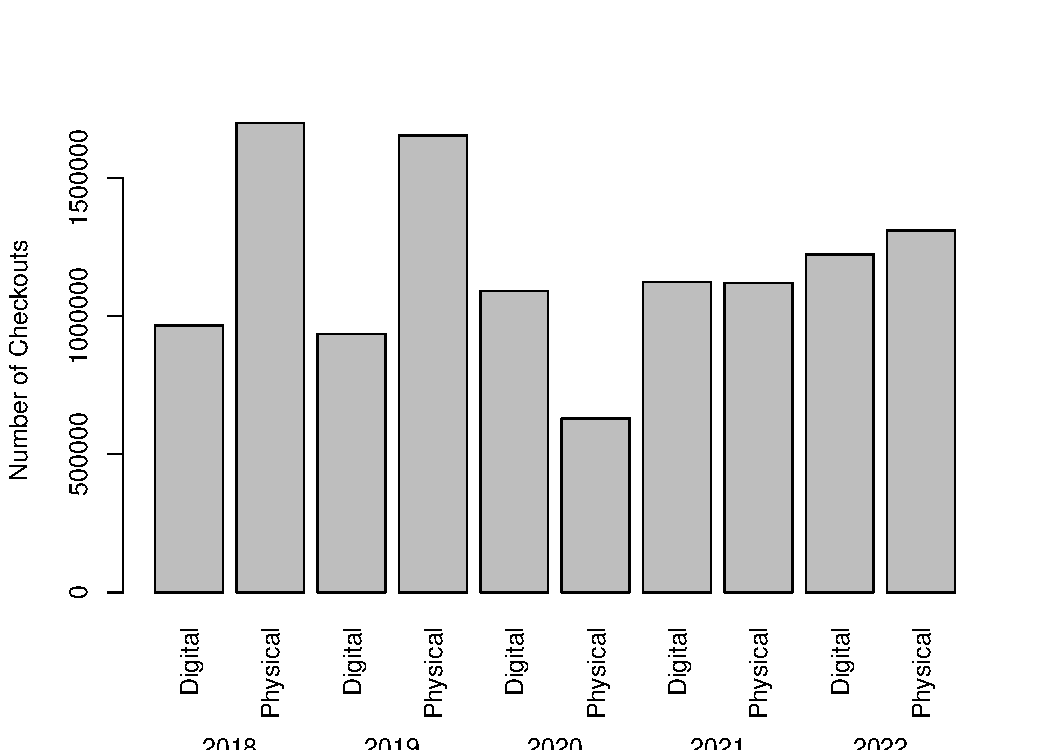
\includegraphics[width=\maxwidth]{figure/plot1-1} 
\end{knitrout}
  \end{center}
\caption{Number of Checkouts by Usage Class (Physical or Digital) per Year from 2018 to 2022.}\label{fig:1}
\end{figure}

\subsection{Plot 2: Most Popular Subjects}

Figure \ref{fig:2} shows the seven most popular book subjects of all books checked out between 2018 and 2022 in descending order of frequency. Books can have multiple subjects, such as both "Fiction" and "Literature." Fiction is the most popular topic with a little over 2.5 million occurrences, and Nonfiction had around 1.5 million. This is unsurprising since fiction and nonfiction are broad identifiers. In addition, in this plot, subjects are re-counted when their corresponding book is checked out again.

\begin{figure}[H]
\begin{center}
\begin{knitrout}
\definecolor{shadecolor}{rgb}{0.969, 0.969, 0.969}\color{fgcolor}
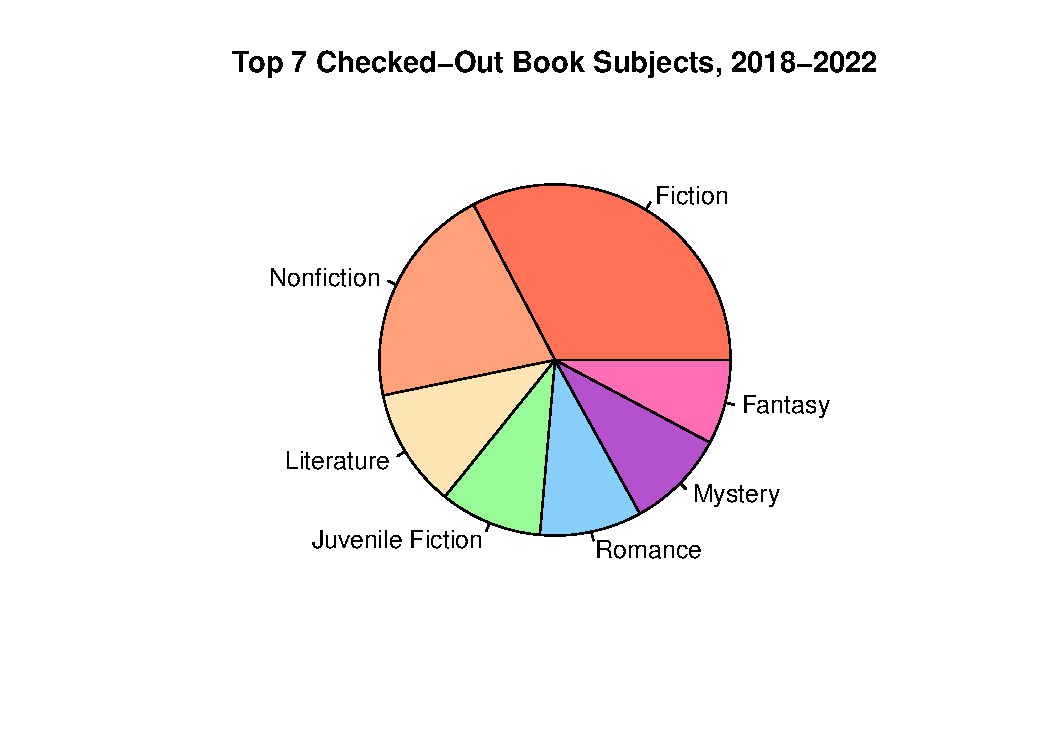
\includegraphics[width=\maxwidth]{figure/plot2-1} 
\end{knitrout}
\end{center}
\caption{Top 7 subjects of all books checked-out from 2018 to 2022.}\label{fig:2}
\end{figure}

\subsection{Plot 3: Most Popular Physical Books}

Figure \ref{fig:3} shows the relative popularity of the seven most popular physical books with checkouts in each year between 2018 and 2022. We use "relative" popularity to signify that these are not necessarily the books that were most popular in each year. Rather, these are the most popular books whose popularity endured over the period in question.

Novels and memoirs dominate, although their popularity curves exhibit a marked difference: popular memoirs (Educated; Becoming) appear to lack the staying power of similarly popular novels (Where the Crawdads Sing; There There; The Overstory). This figure could serve as ground zero for an investigation into the popularity curves and how they vary both within and across generic boundaries.

We also note the curious prevalence of reading lines (A Memoir; a Novel). Reading lines have a long and complex history, beginning with 17th century publishers who sought to delineate new, experimentally-realistic work from older romances and epics. Early 20th century writers, by contrast, often troubled this binary by affixing "a Novel" to works that few readers would deem "realistic." Finally, post-45 American authors and publishers used (and continue to use!) reading lines to assert, aspirationally, that their book belongs among that most "serious" and "literary" in-group: prizewinners. An examination linking reading lines to popularity certainly bears further investigation. 

\begin{figure}[H]
\begin{center}
\begin{knitrout}
\definecolor{shadecolor}{rgb}{0.969, 0.969, 0.969}\color{fgcolor}\begin{kframe}


{\ttfamily\noindent\bfseries\color{errorcolor}{\#\# Error in top\_books\_counts \%>\% group\_by(year) \%>\% mutate(rank = rank(-x)) \%>\% : could not find function "{}\%>\%"{}}}

{\ttfamily\noindent\bfseries\color{errorcolor}{\#\# Error in eval(expr, envir, enclos): object 'book\_positions\_by\_year' not found}}

{\ttfamily\noindent\bfseries\color{errorcolor}{\#\# Error in strsplit(titles, "{} / "{}): object 'titles' not found}}

{\ttfamily\noindent\bfseries\color{errorcolor}{\#\# Error in plot.default(NULL, type = "{}l"{}, col = "{}black"{}, lwd = 1, main = "{}Most Popular Books 2018-2022"{}, : object 'book\_positions\_by\_year' not found}}

{\ttfamily\noindent\bfseries\color{errorcolor}{\#\# Error in eval(expr, envir, enclos): object 'titles' not found}}\end{kframe}
\end{knitrout}
\end{center}
\caption{Relative popularity of the most popular physical books 2018-2022}\label{fig:3}
\end{figure}

\subsection{Plot 4: Prior Year vs. Current Year Popularity}

Figure \ref{fig:4} demonstrates the degree to which current-year popularity is predicted by prior-year popularity for years 2019-2022. We present a log-log plot of current vs. prior popularity and overlay a line of best fit. Prior popularity seems a fair -- though by no means perfect -- predictor of future popularity. Noticeably, there two groups straddle the line of best fit: one with over-predicted popularity and one under-predicted. These groups might be a consequence of the nature of popularity; namely, it's either rising or falling. Or this early analysis could be indentifying two categorically different groups of books: successes and flops. 

\begin{figure}[H]
\begin{center}
\begin{knitrout}
\definecolor{shadecolor}{rgb}{0.969, 0.969, 0.969}\color{fgcolor}\begin{kframe}


{\ttfamily\noindent\bfseries\color{errorcolor}{\#\# Error in title\_counts\_by\_year \%>\% group\_by(title) \%>\% mutate(prev = lag(x, : could not find function "{}\%>\%"{}}}

{\ttfamily\noindent\bfseries\color{errorcolor}{\#\# Error in is.data.frame(data): object 'curr\_prev\_year\_counts' not found}}

{\ttfamily\noindent\bfseries\color{errorcolor}{\#\# Error in plot(curr\_prev\_year\_counts\$prev, curr\_prev\_year\_counts\$curr, : object 'curr\_prev\_year\_counts' not found}}

{\ttfamily\noindent\bfseries\color{errorcolor}{\#\# Error in abline(reg = curr\_prev\_model, col = "{}red"{}): object 'curr\_prev\_model' not found}}\end{kframe}
\end{knitrout}
\end{center}
\caption{Current year vs. prior year checkouts, log-log scale}\label{fig:4}
\end{figure}


\subsection{Plot 5: Normalized Increase in Checkouts between Textbooks vs. all Other Books}

Figure \ref{fig:5} compares the normalized increase from the minimum monthly checkouts between textbooks and all other books including the years 2018-2022. The Q-Q plot compares the quantiles of the total checkouts for each month from the two book categories along with a line of best fit. While both sets of data seem to be distributed roughly the same, there is a slight increase in textbook checkouts in the summer months leading up to the fall semester that drops off once the fall has started. While this is a good start, future work would inclduing looking more in depth at the difference between years during the COVID-19 pandemic and the years before.

\begin{figure}[H]
\begin{center}
\begin{knitrout}
\definecolor{shadecolor}{rgb}{0.969, 0.969, 0.969}\color{fgcolor}
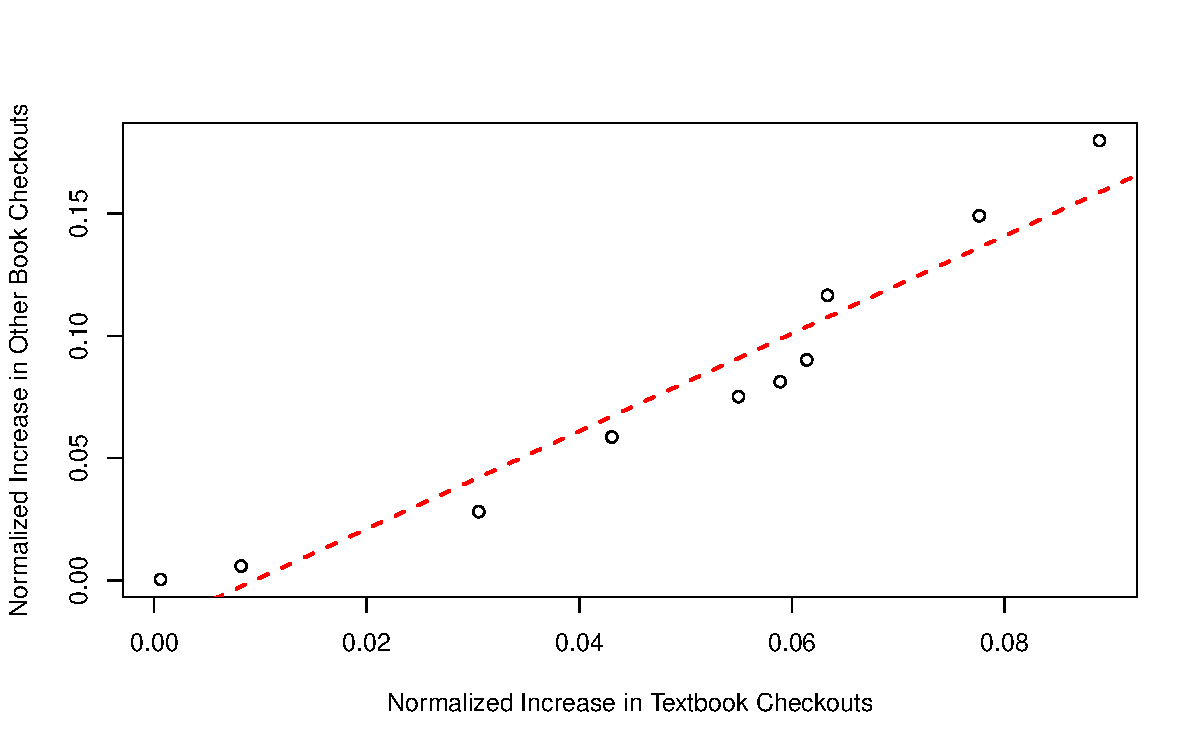
\includegraphics[width=\maxwidth]{figure/plot5-1} 
\end{knitrout}
\end{center}
\caption{Normalized increase in textbook checkouts compared to all other books}\label{fig:5}
\end{figure}

\end{document}
